\documentclass{article}
\usepackage[paperwidth=360pt,paperheight=190pt,margin=0pt,noheadfoot]{geometry}
\usepackage{tikz}
\usetikzlibrary{calc}

\definecolor{ink}{RGB}{28,41,56}
\definecolor{axis}{RGB}{100,116,139}
\definecolor{grid}{RGB}{203,213,225}
\definecolor{curve}{RGB}{30,64,175}
\definecolor{teal}{RGB}{13,148,136}
\definecolor{tealfill}{RGB}{176,227,219}
% Integral diagrams use exactly one semantic palette: blue for the
% lower-only part, yellow for the upper-only (or still unresolved) part, and
% green for their common part.  The common part is explicit rather than an
% alpha blend, so the three meanings stay distinct after GIF quantization.
\definecolor{blue}{RGB}{0,114,178}
\definecolor{bluefill}{RGB}{86,180,233}
\definecolor{yellow}{RGB}{230,159,0}
\definecolor{yellowfill}{RGB}{255,218,102}
\definecolor{green}{RGB}{0,128,84}
\definecolor{greenfill}{RGB}{89,190,142}
\definecolor{orange}{RGB}{234,88,12}
\definecolor{orangefill}{RGB}{254,215,170}
\definecolor{purple}{RGB}{126,34,206}
\definecolor{yellowedge}{RGB}{202,138,4}
\definecolor{projection}{RGB}{148,163,184}
\colorlet{under}{blue}
\colorlet{underfill}{bluefill}
\colorlet{over}{yellow}
\colorlet{overfill}{yellowfill}
\colorlet{shared}{green}
\colorlet{sharedfill}{greenfill}
\colorlet{gap}{yellow}
\colorlet{gapfill}{yellowfill}

\pagestyle{empty}
\setlength\parindent{0pt}
\setlength\topskip{0pt}
\begin{document}
\noindent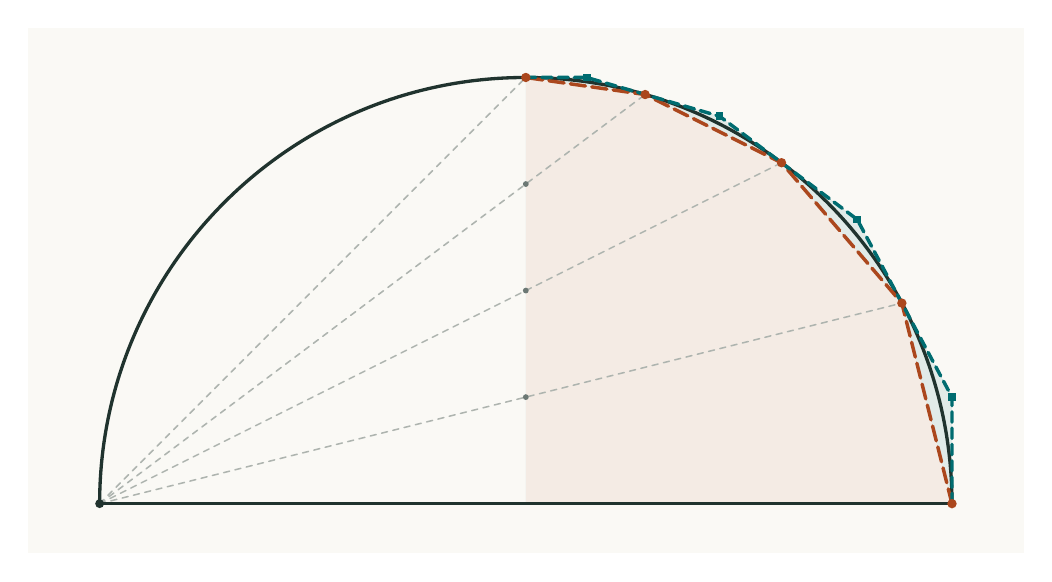
\begin{tikzpicture}[baseline=(current bounding box.north),x=1pt,y=1pt,line cap=round,line join=round]
\useasboundingbox (0,0) rectangle (360,190);
\definecolor{paper}{HTML}{FAF9F5}
\definecolor{semicircle}{HTML}{20332E}
\definecolor{lowerbound}{HTML}{AB471D}
\definecolor{upperbound}{HTML}{006C70}
\fill[paper] (0,0) rectangle (360,190);
\fill[upperbound!10!paper] (180,18) -- (334,18) -- (334,56.5) -- (299.7778,120.6667) -- (250,158) -- (202,172) -- (180,172) -- cycle;
\fill[lowerbound!8!paper] (180,18) -- (334,18) -- (315.8824,90.4706) -- (272.4,141.2) -- (223.12,165.84) -- (180,172) -- cycle;
\draw[semicircle!35!paper,line width=.55pt,dash pattern=on 2.2pt off 2pt] (26,18) -- (315.8824,90.4706);
\fill[semicircle!65!paper] (180,56.5) circle[radius=1.05pt];
\draw[semicircle!35!paper,line width=.55pt,dash pattern=on 2.2pt off 2pt] (26,18) -- (272.4,141.2);
\fill[semicircle!65!paper] (180,95) circle[radius=1.05pt];
\draw[semicircle!35!paper,line width=.55pt,dash pattern=on 2.2pt off 2pt] (26,18) -- (223.12,165.84);
\fill[semicircle!65!paper] (180,133.5) circle[radius=1.05pt];
\draw[semicircle!35!paper,line width=.55pt,dash pattern=on 2.2pt off 2pt] (26,18) -- (180,172);
\fill[semicircle!65!paper] (180,172) circle[radius=1.05pt];
\draw[semicircle,line width=.85pt] (26,18) -- (334,18);
\draw[semicircle,line width=1.2pt] (334,18) arc[start angle=0,end angle=180,radius=154pt];
\draw[lowerbound,line width=1.25pt,dash pattern=on 5.5pt off 2.3pt] (334,18) -- (315.8824,90.4706) -- (272.4,141.2) -- (223.12,165.84) -- (180,172);
\draw[upperbound,line width=1.25pt,dash pattern=on 3.7pt off 2.2pt] (334,18) -- (334,56.5) -- (299.7778,120.6667) -- (250,158) -- (202,172) -- (180,172);
\fill[semicircle] (26,18) circle[radius=1.6pt];
\fill[lowerbound] (334,18) circle[radius=1.7pt];
\fill[lowerbound] (315.8824,90.4706) circle[radius=1.7pt];
\fill[lowerbound] (272.4,141.2) circle[radius=1.7pt];
\fill[lowerbound] (223.12,165.84) circle[radius=1.7pt];
\fill[lowerbound] (180,172) circle[radius=1.7pt];
\fill[upperbound] (332.6,55.1) rectangle (335.4,57.9);
\fill[upperbound] (298.3778,119.2667) rectangle (301.1778,122.0667);
\fill[upperbound] (248.6,156.6) rectangle (251.4,159.4);
\fill[upperbound] (200.6,170.6) rectangle (203.4,173.4);
\end{tikzpicture}
\end{document}
